% The same AA tree, laid out by level; horizontal red links preserve the level.
% Editable source for this diagram. From this directory, regenerate with:
% latex -interaction=nonstopmode -halt-on-error aa-tree-4.tex
% dvisvgm --no-fonts --exact --bbox=papersize --output=aa-tree-4.svg aa-tree-4.dvi
\documentclass[tikz,border=2pt]{standalone}
\usepackage{lmodern}
\usepackage{tikz}
\usetikzlibrary{arrows.meta,backgrounds,shapes.geometric,patterns}
\definecolor{linkred}{HTML}{B5240A}
\definecolor{noteBlue}{HTML}{0067A5}
\definecolor{softgreen}{HTML}{D8EAD0}
\definecolor{softpurple}{HTML}{D9D1E8}
\definecolor{softpink}{HTML}{F5CECF}
\definecolor{softyellow}{HTML}{FFF2C9}
\begin{document}
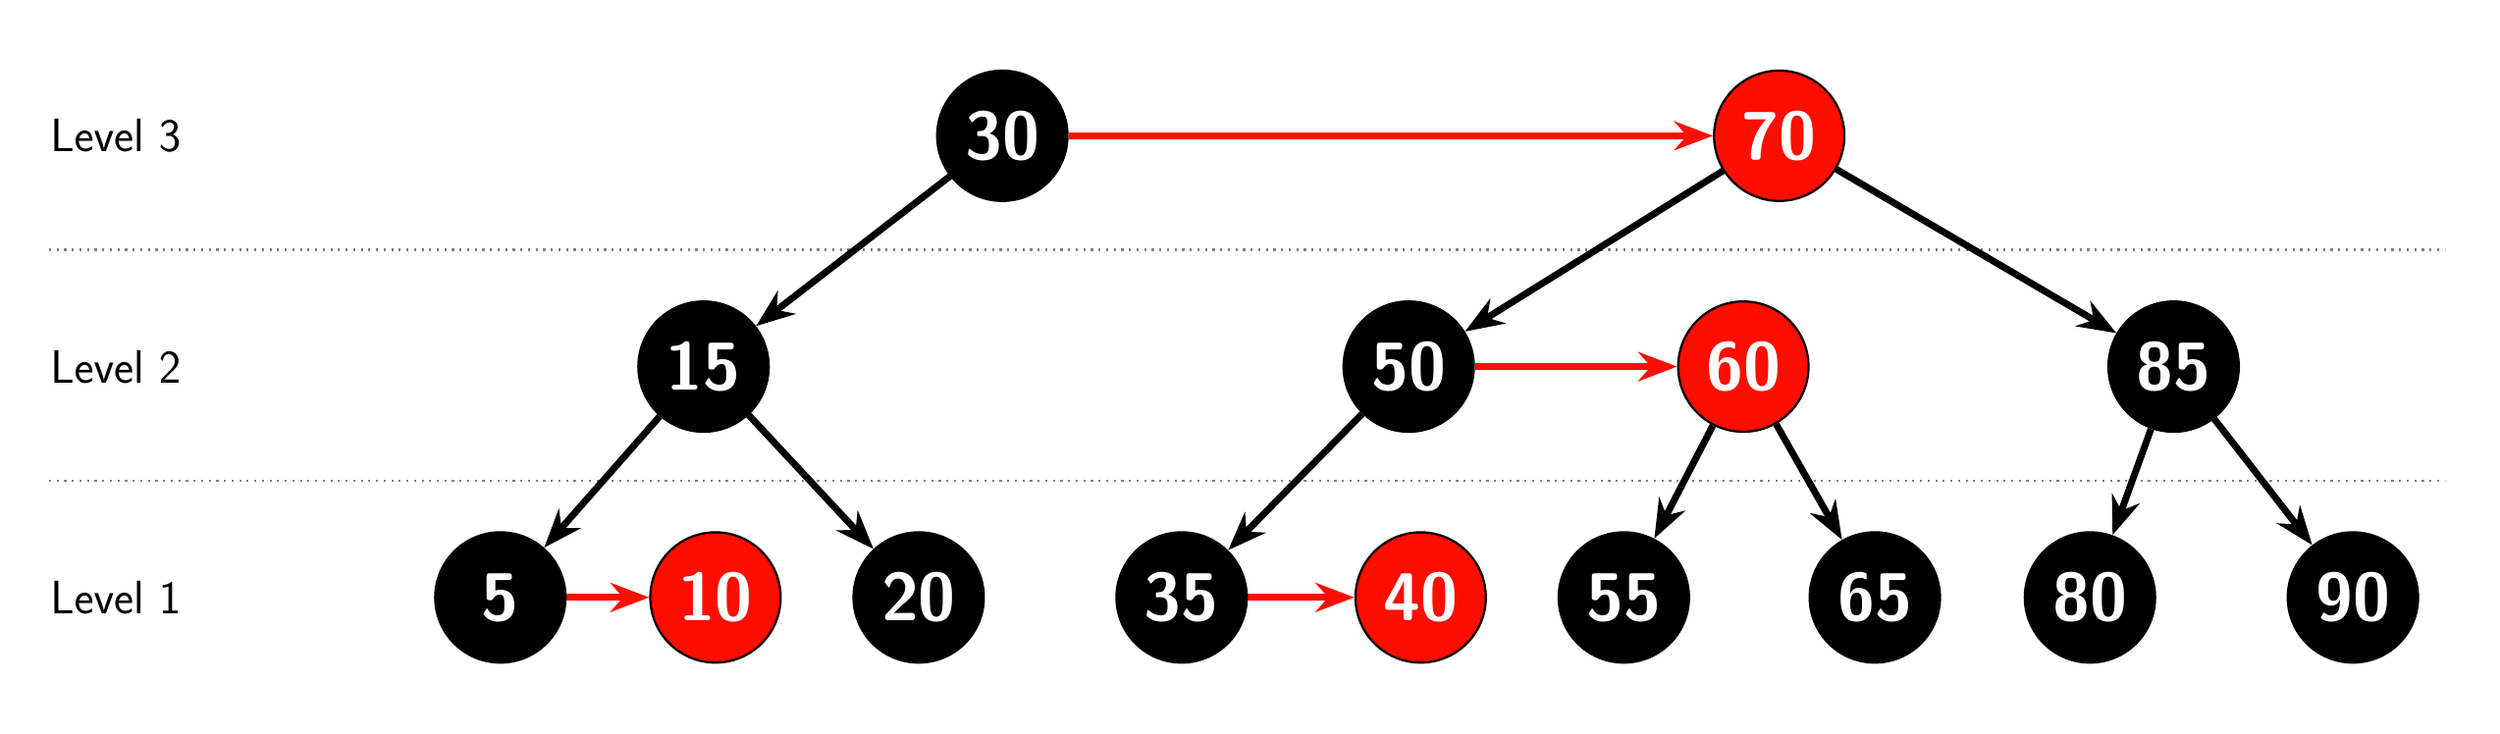
\begin{tikzpicture}[x=1pt,y=-1pt,>=Stealth,line cap=round,line join=round]
\path[use as bounding box] (0,0) rectangle (900,250);
\begin{scope}[on background layer]
\draw[draw=gray,line width=0.8pt,dotted] (8,82) -- (890,82);
\draw[draw=gray,line width=0.8pt,dotted] (8,167) -- (890,167);
\end{scope}
\node[circle,draw=black,fill=black,text=white,minimum size=48pt,inner sep=0pt,line width=0.8pt,font=\sffamily\fontsize{23}{27.6}\selectfont,font=\sffamily\bfseries\fontsize{23}{27}\selectfont] (n30) at (359.0,40) {30};
\node[circle,draw=black,fill=red!90!orange,text=white,minimum size=48pt,inner sep=0pt,line width=0.8pt,font=\sffamily\fontsize{23}{27.6}\selectfont,font=\sffamily\bfseries\fontsize{23}{27}\selectfont] (n70) at (645.0,40) {70};
\node[circle,draw=black,fill=black,text=white,minimum size=48pt,inner sep=0pt,line width=0.8pt,font=\sffamily\fontsize{23}{27.6}\selectfont,font=\sffamily\bfseries\fontsize{23}{27}\selectfont] (n15) at (249.0,125) {15};
\node[circle,draw=black,fill=black,text=white,minimum size=48pt,inner sep=0pt,line width=0.8pt,font=\sffamily\fontsize{23}{27.6}\selectfont,font=\sffamily\bfseries\fontsize{23}{27}\selectfont] (n50) at (508.6,125) {50};
\node[circle,draw=black,fill=red!90!orange,text=white,minimum size=48pt,inner sep=0pt,line width=0.8pt,font=\sffamily\fontsize{23}{27.6}\selectfont,font=\sffamily\bfseries\fontsize{23}{27}\selectfont] (n60) at (631.8,125) {60};
\node[circle,draw=black,fill=black,text=white,minimum size=48pt,inner sep=0pt,line width=0.8pt,font=\sffamily\fontsize{23}{27.6}\selectfont,font=\sffamily\bfseries\fontsize{23}{27}\selectfont] (n85) at (790.2,125) {85};
\node[circle,draw=black,fill=black,text=white,minimum size=48pt,inner sep=0pt,line width=0.8pt,font=\sffamily\fontsize{23}{27.6}\selectfont,font=\sffamily\bfseries\fontsize{23}{27}\selectfont] (n5) at (174.2,210) {5};
\node[circle,draw=black,fill=red!90!orange,text=white,minimum size=48pt,inner sep=0pt,line width=0.8pt,font=\sffamily\fontsize{23}{27.6}\selectfont,font=\sffamily\bfseries\fontsize{23}{27}\selectfont] (n10) at (253.4,210) {10};
\node[circle,draw=black,fill=black,text=white,minimum size=48pt,inner sep=0pt,line width=0.8pt,font=\sffamily\fontsize{23}{27.6}\selectfont,font=\sffamily\bfseries\fontsize{23}{27}\selectfont] (n20) at (328.2,210) {20};
\node[circle,draw=black,fill=black,text=white,minimum size=48pt,inner sep=0pt,line width=0.8pt,font=\sffamily\fontsize{23}{27.6}\selectfont,font=\sffamily\bfseries\fontsize{23}{27}\selectfont] (n35) at (425.0,210) {35};
\node[circle,draw=black,fill=red!90!orange,text=white,minimum size=48pt,inner sep=0pt,line width=0.8pt,font=\sffamily\fontsize{23}{27.6}\selectfont,font=\sffamily\bfseries\fontsize{23}{27}\selectfont] (n40) at (513.0,210) {40};
\node[circle,draw=black,fill=black,text=white,minimum size=48pt,inner sep=0pt,line width=0.8pt,font=\sffamily\fontsize{23}{27.6}\selectfont,font=\sffamily\bfseries\fontsize{23}{27}\selectfont] (n55) at (587.8,210) {55};
\node[circle,draw=black,fill=black,text=white,minimum size=48pt,inner sep=0pt,line width=0.8pt,font=\sffamily\fontsize{23}{27.6}\selectfont,font=\sffamily\bfseries\fontsize{23}{27}\selectfont] (n65) at (680.2,210) {65};
\node[circle,draw=black,fill=black,text=white,minimum size=48pt,inner sep=0pt,line width=0.8pt,font=\sffamily\fontsize{23}{27.6}\selectfont,font=\sffamily\bfseries\fontsize{23}{27}\selectfont] (n80) at (759.4,210) {80};
\node[circle,draw=black,fill=black,text=white,minimum size=48pt,inner sep=0pt,line width=0.8pt,font=\sffamily\fontsize{23}{27.6}\selectfont,font=\sffamily\bfseries\fontsize{23}{27}\selectfont] (n90) at (856.2,210) {90};
\begin{scope}[on background layer]
\draw[draw=black,line width=2.5pt,->] (n30) -- (n15);
\draw[draw=red!90!orange,line width=2.5pt,->] (n30) -- (n70);
\draw[draw=black,line width=2.5pt,->] (n15) -- (n5);
\draw[draw=black,line width=2.5pt,->] (n15) -- (n20);
\draw[draw=red!90!orange,line width=2.5pt,->] (n5) -- (n10);
\draw[draw=black,line width=2.5pt,->] (n70) -- (n50);
\draw[draw=black,line width=2.5pt,->] (n70) -- (n85);
\draw[draw=black,line width=2.5pt,->] (n50) -- (n35);
\draw[draw=red!90!orange,line width=2.5pt,->] (n50) -- (n60);
\draw[draw=red!90!orange,line width=2.5pt,->] (n35) -- (n40);
\draw[draw=black,line width=2.5pt,->] (n60) -- (n55);
\draw[draw=black,line width=2.5pt,->] (n60) -- (n65);
\draw[draw=black,line width=2.5pt,->] (n85) -- (n80);
\draw[draw=black,line width=2.5pt,->] (n85) -- (n90);
\end{scope}
\node[anchor=west,text=black,font=\sffamily\fontsize{18}{21.6}\selectfont] at (5,40) {Level 3};
\node[anchor=west,text=black,font=\sffamily\fontsize{18}{21.6}\selectfont] at (5,125) {Level 2};
\node[anchor=west,text=black,font=\sffamily\fontsize{18}{21.6}\selectfont] at (5,210) {Level 1};
\end{tikzpicture}
\end{document}
